%!TEX root = ../../paper.tex
\begin{table}
	\centering
	%!TEX root = ../../paper.tex

\begin{tabular}{l*{2}{S[scientific-notation=true, round-mode=places,round-precision=3]}}
\toprule
~ 				& \multicolumn{2}{c}{Estimator}\\ \cmidrule{2-3}
Set				& {\mbe}					& {\sambe}	\\
\midrule
\ferdosiOne		& 8.30580618349064E-09		&  8.9087329457441E-09 \\
\baakmanOne		& 1.49022877061299E-08		&  1.5398737157543E-08 \\	
\baakmanFour	& 2.93709420107411E-08		&  2.9634323205557E-08 \\	
\baakmanFive	& 5.57179476550916E-08		&  5.5847473903432E-08 \\	
\bottomrule
\end{tabular}
	\caption{Performance of the symmetric and the shape-adaptive Modified Breiman Estimator on dataset \ferdosiTwo through \baakmanThree.} 	
	\label{tab:results:multiSphere:mse}
\end{table}

% What does the section do
In this section we present the results of the two estimators on dataset \ferdosiTwo, \baakmanTwo, \ferdosiThree, and \baakmanThree.
% MSE
	% GENERAL
	Based on the small differences between the \mses of the estimators in \cref{tab:results:multiSphere:mse} they perform comparably. 
	% FERDOSI 2 
		% COMPONENT 1 MBE MSE 1.385919090205819e-07 (            ) SAMBE MSE 1.384478742850174e-07 (            )
		% COMPONENT 2 MBE MSE 1.313643043640668e-08 (1.629142e-08) SAMBE MSE 1.302177563181053e-08 (1.742749e-08)
		% NOISE  	  MBE MSE 2.293851560028409e-11 (            ) SAMBE MSE 2.329767921658432e-11 (            )
	% BAAKMAN 2
		% COMPONENT 1 MBE MSE 1.407069060886291e-07 (            ) SAMBE MSE 1.412169246599802e-07 (            )
		% COMPONENT 2 MBE MSE 1.367299679831388e-08 (1.682701e-08) SAMBE MSE 1.378034105739574e-08 (1.825202e-08)
		% NOISE 	  MBE MSE 3.497662493386784e-11 (            ) SAMBE MSE 3.920943401183576e-11	(            )
	% FERDOSI 3	
		% COMPONENT 1 MBE MSE 2.390294620096452e-06 SAMBE MSE 2.466705633403533e-06
		% COMPONENT 2 MBE MSE 1.188881378312256e-08 SAMBE MSE 1.231201873705999e-08
		% COMPONENT 3 MBE MSE 2.373920131423336e-05 SAMBE MSE 2.418690791957957e-05
		% COMPONENT 4 MBE MSE 1.113882923683008e-07 SAMBE MSE 1.152633135516966e-07
		% NOISE 	  MBE MSE 4.320565280514733e-10 SAMBE MSE 4.461773022571117e-10
	% BAAKMAN 3
		% COMPONENT 1 MBE MSE 2.329212432941902e-06 SAMBE MSE 2.391586354071871e-06
		% COMPONENT 2 MBE MSE 1.748202359601445e-08 SAMBE MSE 1.764561034215026e-08
		% COMPONENT 3 MBE MSE 2.265532341806348e-05 SAMBE MSE 2.316257978616503e-05
		% COMPONENT 4 MBE MSE 1.312379885278773e-07 SAMBE MSE 1.339883658098755e-07
		% NOISE 	  MBE MSE 3.916881734521594e-10 SAMBE MSE 4.028048478164317e-10
	% FOCUS ON COMPONENTS
	Comparing the \MSE between components and estimators within data sets yields no differences. However within data sets the differences in \mses between components are quite large.
	% FERDOSI 2 & BAAKMAN 2
	Within dataset \ferdosiTwo and \baakmanTwo both estimators perform significantly better on the component with higher values on the diagonal of its covariance matrix, \ie `Trivariate Gaussian 2'.
	% FERDOSI 3 & BAAKMAN 3
	In data set \ferdosiThree and \baakmanThree both estimators show a negative correlation between the eigenvalues of the covariance matrix of that component and the \MSE of points sampled from that component. Additionally, contrary to our expectation the symmetric estimator performed better on dataset \baakmanThree, than on the symmetric set it was derived from.

% PLOTS
	% GENERAL: TWO SPHERES
	\begin{figure}
		\centering
		%!TEX root = ../../paper.tex

% Ferdosi 2, MBE
\begin{subfigure}{0.23\textwidth}
	\centering
	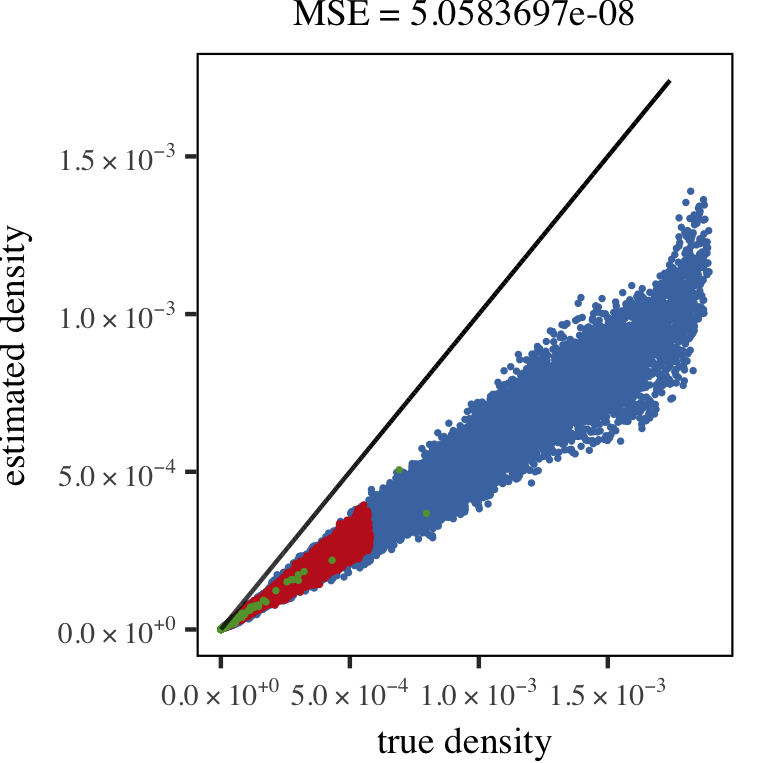
\includegraphics[keepaspectratio=true, width=\textwidth, height=0.23\textheight]{result/img/results_ferdosi_2_60000_mbe_silverman}
	\caption{Set \ferdosiTwo, \mbe}
	\label{fig:results:multisphere:mbe:ferdosi2}
\end{subfigure}
% Baakman 2, MBE
\begin{subfigure}{0.23\textwidth}
	\centering
	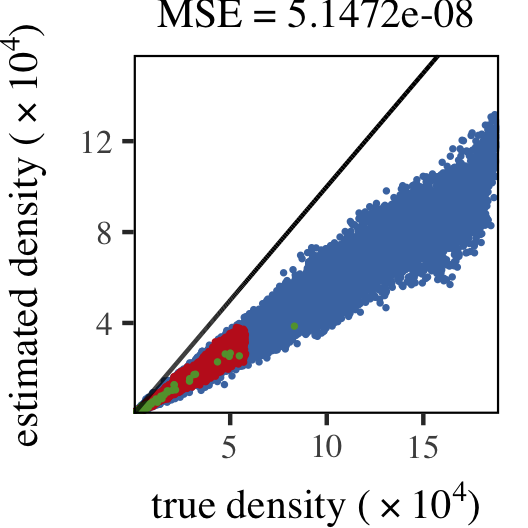
\includegraphics[keepaspectratio=true, width=\textwidth, height=0.23\textheight]{result/img/results_baakman_2_60000_mbe_silverman}
	\caption{Set \baakmanTwo, \mbe}
	\label{fig:results:multisphere:mbe:baakman2}
\end{subfigure}
% Ferdosi 2, SAMBE
\begin{subfigure}{0.23\textwidth}
	\centering
	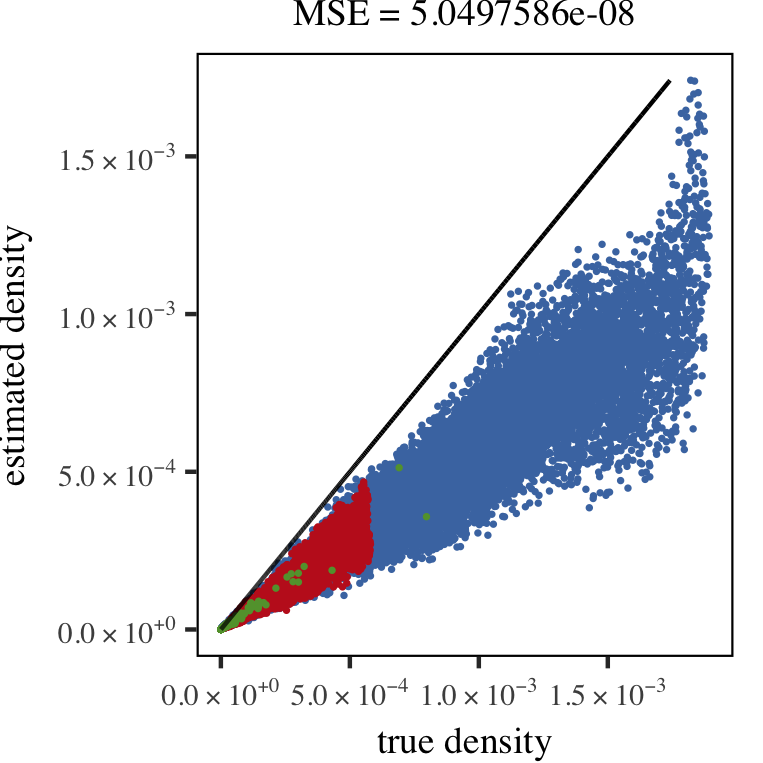
\includegraphics[keepaspectratio=true, width=\textwidth, height=0.23\textheight]{result/img/results_ferdosi_2_60000_sambe_silverman}
	\caption{Set \ferdosiTwo, \sambe}
	\label{fig:results:multisphere:sambe:ferdosi2}
\end{subfigure}
% Baakman 2, SAMBE
\begin{subfigure}{0.23\textwidth}
	\centering
	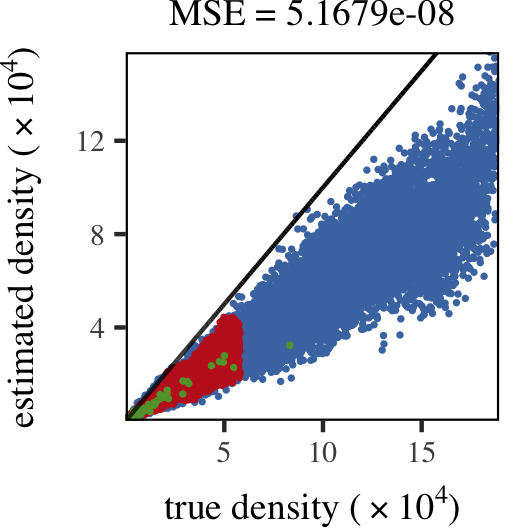
\includegraphics[keepaspectratio=true, width=\textwidth, height=0.23\textheight]{result/img/results_baakman_2_60000_sambe_silverman}
	\caption{Set \baakmanTwo, \sambe}
	\label{fig:results:multisphere:sambe:baakman2}
\end{subfigure}
		\caption{Plots of the true versus estimated density of datasets \ferdosiTwo and \baakmanTwo for the shape-adaptive and the symmetric Modified Breiman Estimator.}
		\label{fig:results:multiSphere:two:comparativePlots}
	\end{figure}
	%
	\Cref{fig:results:multiSphere:two:comparativePlots} shows the estimated density as a function of the known density for both estimators for the datasets with two Gaussian components. These plots show that irrespective of the type of kernel used the density is underestimated, \mbe more so than \sambe. Furthermore using shape-adaptive kernels results in a larger variation in estimated densities than the use of symmetric kernels. 
	% FERDOSI 2
	% BAAKMAN 2	
	% FOCUS ON COMPONENTS
		% SAMBE seems better on red comonent
		Comparing the results of \sambe with those of \mbe in \cref{fig:results:multiSphere:three:comparativePlots} suggest that \sambe hardly underestimates the densities of the most anisotropic component, \ie `Trivariate Gaussian 2' in dataset \ferdosiTwo and \baakmanTwo. However the difference in \mse of this component between \mbe and \sambe is pretty small. The large difference in standard deviation of the squared error between estimators on this component suggests that the seemingly better performance of the shape-adaptive estimator is due to its higher spread of estimated densities.
		% Better performance on 
		Furthermore the \mses of the individual components of dataset \ferdosiTwo and \baakmanThree show that both estimators perform worse on components with covariance matrices that have low eigenvalues, \eg `Trivariate Gaussian 1'.
	%		
	% GENERAL: FOUR SPHERES
	\begin{figure}
		\centering
		%!TEX root = ../../paper.tex

% Ferdosi 3, MBE
\begin{subfigure}{0.33\textwidth}
	\centering
	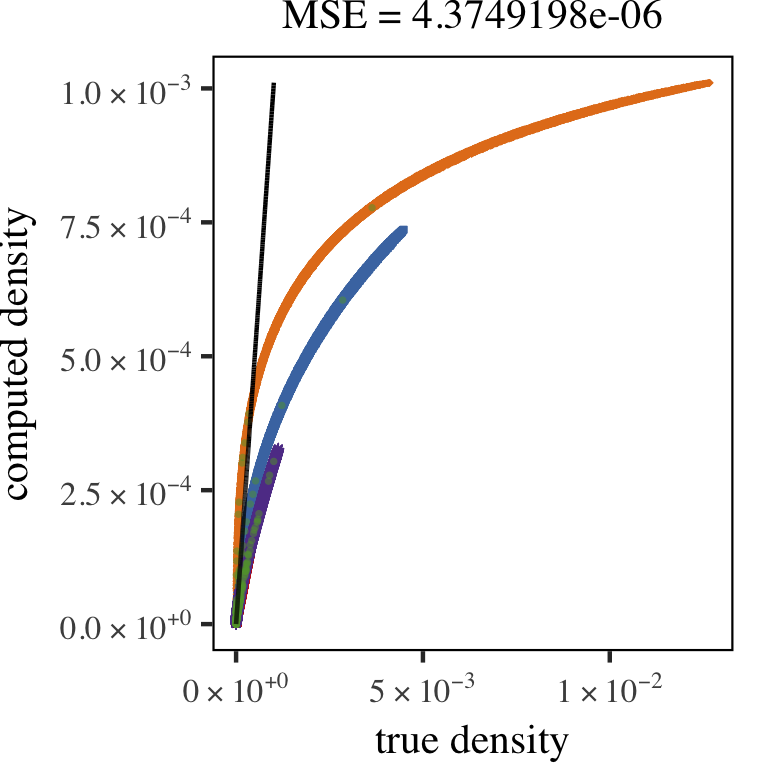
\includegraphics[keepaspectratio=true, width=\textwidth, height=0.23\textheight]{result/img/results_ferdosi_3_120000_mbe_silverman.png}
	\caption{Set \ferdosiThree, \mbe}
	\label{fig:results:multisphere:mbe:ferdosi3}
\end{subfigure}
% Baakman 3, MBE
\begin{subfigure}{0.33\textwidth}
	\centering
	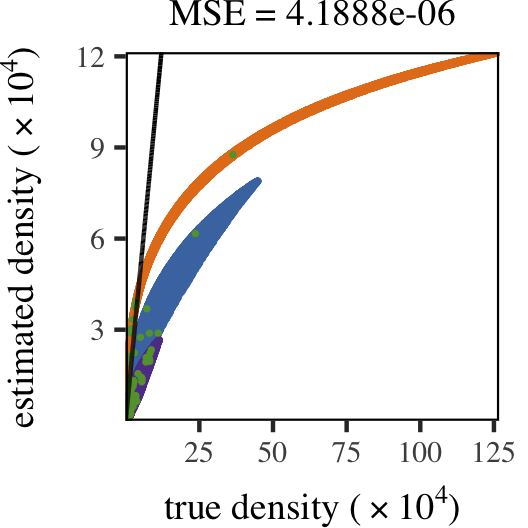
\includegraphics[keepaspectratio=true, width=\textwidth, height=0.23\textheight]{result/img/results_baakman_3_120000_mbe_silverman}
	\caption{Set \baakmanThree, \mbe}
	\label{fig:results:multisphere:mbe:baakman3}
\end{subfigure}	
% Ferdosi 3, SAMBE
\begin{subfigure}{0.33\textwidth}
	\centering
	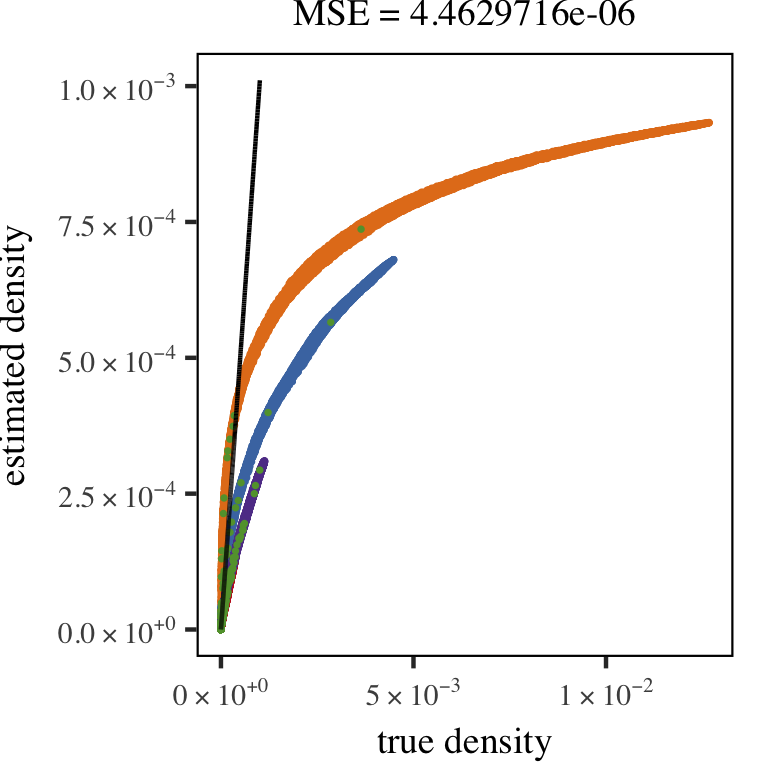
\includegraphics[keepaspectratio=true, width=\textwidth, height=0.23\textheight]{result/img/results_ferdosi_3_120000_sambe_silverman}
	\caption{Set \ferdosiThree, \sambe}
	\label{fig:results:multisphere:sambe:ferdosi3}
\end{subfigure}
% Baakman 3, SAMBE
\begin{subfigure}{0.33\textwidth}
	\centering
	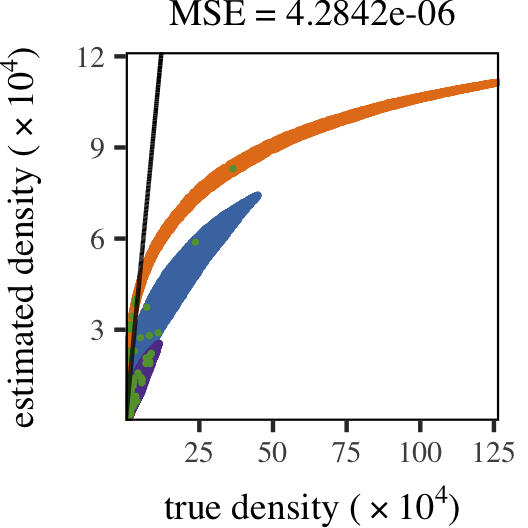
\includegraphics[keepaspectratio=true, width=\textwidth, height=0.23\textheight]{result/img/results_baakman_3_120000_sambe_silverman}
	\caption{Set \baakmanThree, \sambe}
	\label{fig:results:multisphere:sambe:baakman3}
\end{subfigure}	
		\caption{The estimated density as a function of the true density for dataset \ferdosiThree and \baakmanThree, for both \mbe and \sambe.}
		\label{fig:results:multiSphere:three:comparativePlots}
	\end{figure}
	%
	The plots in \cref{fig:results:multiSphere:three:comparativePlots} confirm the large difference in performance between datasets with two and four Gaussian components observed in \cref{tab:results:multiSphere:mse}. Moreover they show that both \mbe and \sambe underestimate densities, especially on the points whose known density is high. In \cref{fig:results:multiSphere:three:comparativePlots} we also observe the larger spread of densities estimated by \sambe, compared to those estimated by \mbe.
	% FERDOSI 3	
	% BAAKMAN 3
	% FOCUS ON COMPONENTS

\todo[inline]{hier verder gaan met reviews}
% ANISOTROPY
	\begin{table*}
		\centering
		%!TEX root = ../../paper.tex

% \sisetup{
% 	table-format=1.3e+1,
% 	scientific-notation=true, 
% 	table-number-alignment=center,
% }

% Mean and SD in single column
% \begin{tabular}{@{}c*{6}{c}@{}}
% \toprule
% ~				& Full Set 												& \legendComponentOne Gaussian 1						& \legendComponentTwo Gaussian 2						& \legendComponentThree Gaussian 3						& \legendComponentFour Gaussian 4					 	&  \legendComponentNoise Noise\\
% \midrule
% %
% \ferdosiTwo		& \meanSD{1.504005042371507e+00}{5.309582791641542e-01} & \meanSD{1.320121582169093e+00}{1.749869852989719e-01} & \meanSD{1.304784013773833e+00}{1.427734068384871e-01} & ~ 													& ~ 													& \meanSD{1.890276960903559e+00}{7.587403345342156e-01}\\
% \baakmanTwo 	& \meanSD{1.614716145373154e+00}{5.702499690627806e-01} & \meanSD{1.407377455694081e+00}{2.782480127488867e-01} & \meanSD{1.491043432778090e+00}{3.453168397321122e-01}	& ~ 													& ~ 													& \meanSD{11.948464282370670e+00}{7.826307984091438e-01}\\
% \ferdosiThree	& \meanSD{1.460357930082488e+00}{5.507084955708148e-01} & \meanSD{1.294023549845817e+00}{1.889517285607608e-01} & \meanSD{1.265946347671562e+00}{1.301150512342848e-01} & \meanSD{1.291829938425150e+00}{2.103396722315814e-01} & \meanSD{1.275739356043035e+00}{1.654855348814119e-01} & \meanSD{1.819950324176552e+00}{8.111641695146756e-01} \\
% \baakmanThree 	& \meanSD{1.532493079967588e+00}{5.713672219810757e-01} & \meanSD{1.314980484677339e+00}{2.190657831683435e-01} & \meanSD{1.487242917765238e+00}{3.393090417977690e-01} & \meanSD{1.291829938425150e+00}{2.103396722315814e-01} & \meanSD{1.396015162355687e+00}{2.851380764085146e-01} & \meanSD{1.854880861700560e+00}{8.195085323228068e-01}\\
% %
% \bottomrule
% \end{tabular}

\small
\sisetup{
	table-format=1.4,
	scientific-notation=fixed,
	table-number-alignment=center,
	fixed-exponent=0,
	round-mode=figures,
	round-precision=4
}


\begin{tabular}{@{}c*{12}{S}@{}}
\toprule
 				& \multicolumn{2}{c}{~} 						& \multicolumn{2}{c}{\legendComponentOne Gaussian 1} 	& \multicolumn{2}{c}{\legendComponentTwo Gaussian 2}	& \multicolumn{2}{c}{\legendComponentThree Gaussian 3}	& \multicolumn{2}{c}{\legendComponentFour Gaussian 4}	& \multicolumn{2}{c}{\legendComponentNoise Noise} \\
															  	\cmidrule(lr){4-5}							  				\cmidrule(lr){6-7}							  			\cmidrule(lr){8-9} 							  			\cmidrule(lr){10-11} 							  \cmidrule(lr){12-13}
~				& {\mean}				& {\SD}			& {\mean}				 & {\SD}			& {\mean}				 & {\SD}			 & {\mean}				& {\SD}			& {\mean}				& {\SD}			& {\mean}					& {\SD}\\ 			
\midrule
\ferdosiTwo		& 1.504005042371507e+00 & 5.309582791641542e-01 & 1.320121582169093e+00 & 1.749869852989719e-01 & 1.304784013773833e+00 & 1.427734068384871e-01 &  						&  						& 	 					&  							& 1.890276960903559e+00 	& 7.587403345342156e-01\\
\baakmanTwo 	& 1.614716145373154e+00 & 5.702499690627806e-01 & 1.407377455694081e+00 & 2.782480127488867e-01 & 1.491043432778090e+00 & 3.453168397321122e-01 &  						&  						& 	 					&  							& 1.948464282370670e+00 	& 7.826307984091438e-01\\
\ferdosiThree 	& 1.460357930082488e+00 & 5.507084955708148e-01 & 1.294023549845817e+00 & 1.889517285607608e-01 & 1.265946347671562e+00 & 1.301150512342848e-01 & 1.291829938425150e+00 & 2.103396722315814e-01 & 1.275739356043035e+00 & 1.654855348814119e-01 	& 1.819950324176552e+00 	& 8.111641695146756e-01 \\
\baakmanThree 	& 1.532493079967588e+00 & 5.713672219810757e-01 & 1.314980484677339e+00 & 2.190657831683435e-01 & 1.487242917765238e+00 & 3.393090417977690e-01 & 1.291829938425150e+00 & 2.103396722315814e-01 & 1.396015162355687e+00 & 2.851380764085146e-01 	& 1.854880861700560e+00 	& 8.195085323228068e-01\\
\bottomrule
\end{tabular}
		\caption{The mean (\mean) and standard deviation (\SD) of the anisotropy of the kernels used for points from the datasets with multiple Gaussians, split per component and for the full dataset.} 	
		\label{tab:results:multiSphere:anisotropy}
	\end{table*}
	% What are we looking at
	\Cref{tab:results:multiSphere:anisotropy} presents the mean and standard deviation of the anisotropy of the kernels used for the points from dataset \ferdosiTwo through \baakmanThree and from their components. 
	% Small differences in anisotropy between F2/F3 and B2/B3
	Although the anisotropy of the kernels used for the datasets with anisotropic Gaussian components is higher on average and more varied than the anisotropy of the kernels used for dataset \ferdosiTwo and \ferdosiThree, the differences are small. 
	% Noise has largest anisotropy
	As in \cref{tab:results:singleSphere:anisotropy} the kernels associated with the points sampled from the component `Uniform random background` have the highest anisotropy, and vary the most in how anisotropic they are. 
	% Positve correlation between mean anisotropy of the kernels and anisotropy of the gaussian components.
	Contrasting the mean anisotropy of the kernels used for points drawn from the different components we find a positive correlation between the mean anisotropy of the kernel and the anisotropy of the Gaussian components. 
	% Positive correlation between anisotropy SD and kernel anisotropy
		% exists for B2
		In the kernels used for dataset \baakmanTwo we observe the same positive correlation between the variation of the anisotropy of the kernels and the anisotropy of the associated kernel as we observed in dataset \baakmanOne, \baakmanFour, and \baakmanFive. 
		% does not occur in B3
		Comparing the standard deviation of the anisotropy of the kernels used for the points sampled from the components of dataset \baakmanThree does not reveal this relation: the densest component, Trivariate Gaussian 3, does not have the highest variation in kernel anisotropy. 
	% ANISOTROPY OF M3 and M4 seems equal for Gaussian 3, is that really the case? 
	One thing that stands out when comparing dataset \ferdosiThree and \baakmanThree in \cref{tab:results:multiSphere:anisotropy} is the lack of difference in the mean and standard deviation in the anisotropy of the kernels associated with the component `Trivariate Gaussian 3'. Reviewing the raw data reveals that the largest difference in anisotropy between any point drawn from that component is \num{3.108624e-15}.

% SUMMARY/CONCLUSION
	% Small differences in MSE between the two datasets
	To summarize the results of the datasets with multiple Gaussian components: we have found that the differences in performance are very small between the two estimators, although \sambe underestimates less than \mbe, the later performs slightly better.
	% Both estimators perform better on denser gaussian components
	Furthermore both estimators show a positive correlation between the density of the Gaussian component and their performance on that component.
	% Differences in anisotropy of the kernels between the F1/F2 and B1/B2 are small. 
	Regarding the anisotropy of the kernels we have found only a small increase between dataset with spherical kernels and dataset \baakmanTwo and \baakmanThree. 
	% Anisotropy is storngest on noise component
	Zeroing in on the components we have observed that the anisotropy of kernels associated with points drawn from the noise is strongest.
	% Positve correlation between mean anisotropy of kernels and anisotropy of the gaussian comonent
	Lastly a positive correlation between the mean anisotropy of the kernels of the points sampled from a component and the anisotropy of the Gaussian those points were drawn from was found. 